\documentclass[12pt]{article}
\usepackage{sbc-template}
\usepackage[utf8]{inputenc}
\usepackage[portuguese]{babel}
\usepackage{lipsum} 
\usepackage{graphicx,url}
\usepackage{amsmath,bm,bbm} 
\usepackage[]{subfigure}
\usepackage{natbib}
\usepackage[colorlinks=true, allcolors=blue]{hyperref} 

\sloppy

\title{Caracterização de imagens PolSAR utilizando Bandt-Pompe PDF e Teoria da Informação}

\author{Danilo Fernandes\inst{1}, Eduarda Chagas\inst{2}, , Roger Almeida\inst{1}}


\address{
  Laboratório de Computação Científica e Análise Numérica (LaCCAN)\\
  Universidade Federal de Alagoas (UFAL) -- Maceio, AL -- Brazil
  \nextinstitute
  Departamento de Ciência da Computação\\
  Universidade Federal de Minas Gerais (UFMG) -- Belo Horizonte, MG -- Brazil
  \email{eduardachagas48@laccan.ufal.br}
}

\begin{document}

\maketitle

\section{Processo de simbolização de Bandt-Pompe para padrões bidimensionais}

Para aplicarmos a simbolização de dados bidimensionais seguindo a metodologia proposta por~\cite{Bandt2002Permutation} devemos considerar, em ambas dimensões, os parâmetros utilizados no algoritmo original. Para fins didáticos, iremos assumir como exemplo uma matriz de tamanho $3$ x $3$, definida a seguir.

\begin{center}
$$
X = \left[
\begin{array}{ccc}
3 & 4 & 8 \\
5 & 6 & 7 \\
2 & 8 & 9 
\end{array}
\right]
$$
\end{center}

O primeiro passo é definir as submatrizes deslizantes e para isso quatro parâmetros são necessários: As dimensões $D_{x}, D_{y} \geq 2$, que são o número de elementos que iram formar os padrões ordinais em ambas dimensões e os delays $\tau _{x}$ e $\tau_{y}$, que informam o quão separados espacialmente estão os símbolos nas duas direções. Neste exemplo, assumiremos $D_{x} = D_{y} = 2$ e $\tau_{x} = \tau_{y} = 1$, obtendo os seguintes quatro particionamentos:

\[
\begin{bmatrix}

A = \left[
\begin{array}{cc}
3 & 4 \\
5 & 6 
\end{array}
\right],

B = \left[
\begin{array}{cc}
4 & 8 \\
6 & 7 
\end{array}
\right],

C = \left[
\begin{array}{cc}
5 & 6 \\
2 & 8 
\end{array}
\right],

D = \left[
\begin{array}{cc}
6 & 7 \\
8 & 9 
\end{array}
\right]

\end{bmatrix}
\]

Após realizar este subdivisão, devemos investigar quais padrões aparecem dentro dos elementos das submatrizes. Para isto, iremos analisar os elementos das destes conjuntos linha por linha, assim $\Pi_{a} = (0,1,2,3)$, pois ao permutar ordenadamente os elementos teremos $a_{1} < a_{2} < a_{3} < a_{4}$. Logo, vamos ter $\Pi_{b} = (0,2,1,3)$, $\Pi_{c} = (3,0,1,2)$ e $\Pi_{d} = (0,1,2,3)$. 

Para todos os padrões ordinais associados a $X$ nós calculamos a distribuição de probabilidade e assim podemos calcular os descritores causais citados anteriormente.

\section{Simulação numérica}

Usamos como fonte de dados uma imagem SAR tirada do Parque Nacional Sierra del Lacandon, Guatemala (adquirido em 10 de abril de 2015), disponível em \url{https://uavsar.jpl.nasa.gov/cgi-bin/product.pl?jobName=Lacand_30202_15043_006_150410_L090_CX_01#dados}. Nossos resultados foram baseados em um pequeno conjunto de amostras correspondentes à banda HHHH desta imagem SAR, podendo ser acessado por: \url{https://drive.google.com/file/d/1-tBmid6Lz_ps_L3OpVVnoR64cENGzR1O/view?usp=sharing}.

Para aplicar as técnicas aqui definidas, consideramos as seguintes configurações nos dados selecionados:

\begin{itemize}
    \item Foram retiradas amostras com dimensão 200x200;
    \item Ao total utilizamos oito regiões, assim definidas:
    \begin{itemize}
        \item Quatro regiões de regiões florestais na Guatemala;
        \item Uma região correspondente a regiões de cultivo na Guatemala;
        \item Três regiões representam regiões terrestres caracterizadas por apresentarem um comportamento não uniforme.
    \end{itemize}
\end{itemize}

Cada amostra é então redimensionada para um conjunto de matrizes obtidas de partições deslizantes da imagem. Assim, testamos o conjunto de valores $(2,3,4,5,6)$ para as dimensões $D_{x}$ e $D_{y}$ das partições geradas. Com o delay usamos os valores $(1,2,3,4,5)$. Para cada partição o processo de simbolização de Bandt-Pompe é realizado, sendo importante salientar que cada dimensão $D_{x}$ e $D_{y}$ leva a $(D_{x}D_{y})!$ possíveis padrões ordinais. 

Enfatizamos que, o uso de rotinas otimizadas implementadas na linguagem \texttt C melhoraram notavelmente o tempo de processamento do experimento, quando comparado com as tradicionais rotinas implementadas anteriormente em \texttt R. Para a adquirir a distribuição de probabilidade de Bandt-Pompe chamamos por meio da interface \texttt{.Call()} uma função inteiramente escrita em \texttt C. Esta função em \texttt C recebe como parâmetros uma matriz contendo as amostras já redimensionadas em particionamentos, a quantidade de colunas que a matriz possui, o que equivale à dimensão $D$, e a quantidade de linhas, que representa a quantidade de casos a serem analisados.

Para cada matriz de representação, calculamos duas medidas de complexidade: Entropia de permutação normalizada $H$ e a Complexidade estatística $C$. Em seguida, aplicamos os valores H e C no plano complexidade-entropia que consiste de uma poderosa ferramenta de discriminação e quantificação das diferentes características dos dados.

\section{Resultados e conclusões}

Sabendo que objetivamos caracterizar as diferentes regiões coletadas em dados SAR, realizamos testes com alguns valores de dimensão e delay. Avaliamos a implicação da modificação destes parâmetros no processo de caracterização destes dados no plano Complexidade-Entropia, como podemos verificar abaixo. 

No gráfico gerado com todas as configurações de dimensões e delays, visualmente representamos as diferentes regiões do seguinte modo:

\begin{itemize}
    \item Regiões florestais -- Triângulos de coloração cinza; 
    \item Regiões de cultivo -- Losangos de coloração azul;
    \item Regiões não uniforme -- Círculos de coloração lilás.
\end{itemize}

Como queremos quantificar e discriminar as características de diferentes tipos de texturas no plano Complexidade-Entropia, os melhores resultados obtidos após essa breve avaliação foram as combinações das seguintes configurações ao aplicar o processo de simbolização de Bandt-Pompe:

\begin{itemize}
    \item $D = 4$ e $\tau = 5$;
    \item $D = 6$ e $\tau = 1$.
\end{itemize}

\begin{figure}[!h]
	\centering
	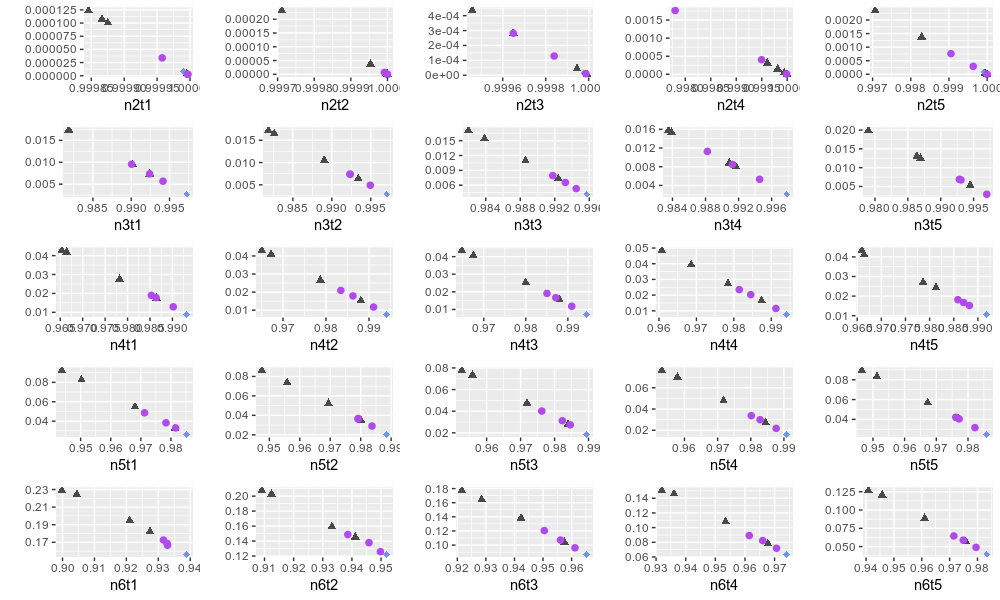
\includegraphics[scale = 0.6]{Rplot.png}        
     \caption{Plano Complexidade-Entropia aplicado as amostras correspondentes à banda HHHH de uma imagem SAR. Verticalmente temos as variações dos valores de delay e horizontalmente dos diferentes valores de dimensão aplicados.}
     \label{fig:Plano}
\end{figure}



\bibliographystyle{agsm}
\bibliography{references.bib}

\end{document}